\documentclass[border=10pt]{standalone}
\usepackage{tikz}
\usepackage{amsmath}
\usetikzlibrary{arrows.meta, calc, patterns, angles, quotes}

\begin{document}

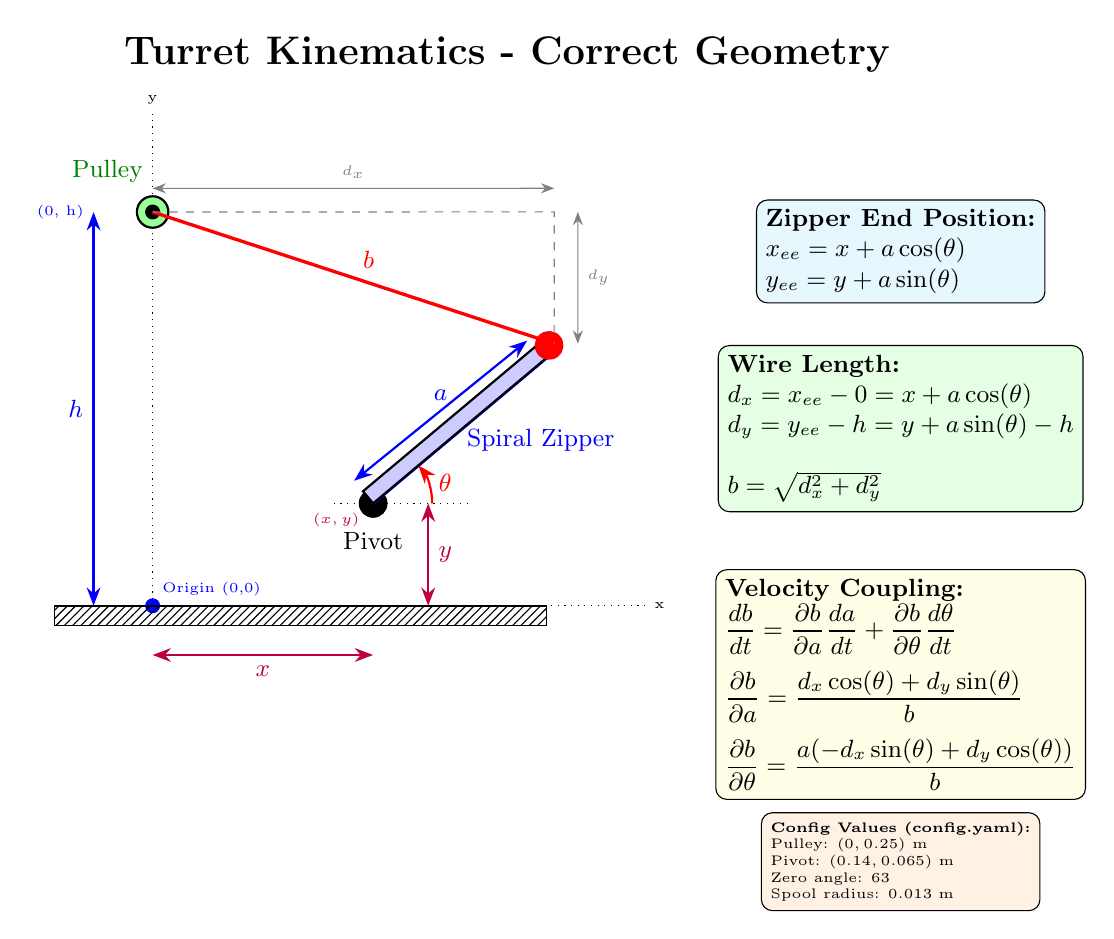
\begin{tikzpicture}[
    scale=2.5,
    >=Stealth,
    fixed/.style={pattern=north east lines}
]

% Define frame origin (0,0)
\coordinate (origin) at (0,0);
\filldraw[blue] (origin) circle (1pt);
\node[above right, font=\tiny, blue] at (origin) {Origin (0,0) };

% Turret frame base
\draw[thick] (-0.5,0) -- (2.0,0);
\draw[fixed] (-0.5,-0.1) rectangle (2.0,0);

% Coordinate axes (dotted reference lines from v3)
\draw[dotted, black] (0,0) -- (2.5,0) node[right, font=\tiny] {x};
\draw[dotted, black] (0,0) -- (0,2.5) node[above, font=\tiny] {y};

% Pulley position (pulley_x=0.0, pulley_y=0.25)
\coordinate (pulley) at (0, 2);
\draw[thick, fill=green!40] (pulley) circle (0.08);
\filldraw[black] (pulley) circle (1pt);
\node[above left, font=\small, text=green!50!black] at ($(pulley) + (0, 0.1)$) {Pulley};

% Vertical dimension for h (pulley_y)
\draw[<->, thick, blue] (-0.3, 0) -- (-0.3, 2)
    node[midway, left, font=\small] {$h$};
\node[left, font=\tiny, blue] at (-0.3, 2) {(0, h)};

% Pivot point position (pivot_x=0.14, pivot_y=0.065)
\coordinate (pivot) at (1.12, 0.52);  % Scaled for visibility
\filldraw[black] (pivot) circle (2pt);
\node[below, font=\small] at ($(pivot) + (0, -0.1)$) {Pivot};

% Dimensions for pivot position
\draw[<->, thick, purple] (0, -0.25) -- (1.12, -0.25)
    node[midway, below, font=\small] {$x$};
\draw[<->, thick, purple] (1.4, 0) -- (1.4, 0.52)
    node[midway, right, font=\small] {$y$};
\node[below left, font=\tiny, purple] at (1.1, 0.52) {$(x, y)$};

% Pitch angle theta (measured from horizontal)
\def\pitchangle{40}
\def\zipperextension{1.2}

% Horizontal reference line through pivot
\draw[dotted, black] ($(pivot) + (-0.2, 0)$) -- ($(pivot) + (0.5, 0)$);

% Pitch angle arc
\draw[thick, ->, red] ($(pivot) + (0.3, 0)$) arc (0:\pitchangle:0.3)
    node[midway, right, font=\small] {$\theta$};

% Spiral zipper at angle theta
\begin{scope}[rotate around={\pitchangle:(pivot)}]
    % Zipper body
    \coordinate (zipper_start) at (pivot);
    \coordinate (zipper_end) at ($(zipper_start) + (\zipperextension, 0)$);

    % Draw zipper as blue bar
    \draw[very thick, blue] (zipper_start) -- (zipper_end);
    \draw[thick, fill=blue!20] (zipper_start) rectangle ($(zipper_end) + (0, 0.08)$);

    % Zipper end (wire attachment point)
    \filldraw[red] ($(zipper_end) + (0, 0.04)$) circle (2pt);

    % Length a
    \draw[<->, thick, blue] ($(zipper_start) + (0, 0.15)$) -- ($(zipper_end) + (-0.07, 0.13)$)
        node[midway, above, font=\small] {$a$};

    % Label
    \node[below right, font=\small, blue] at ($(zipper_start) + (\zipperextension/2, 0.05)$) {Spiral Zipper};
\end{scope}

% Calculate zipper end position in world coordinates
\coordinate (zipper_end_world) at ($(pivot) + ({\zipperextension*cos(\pitchangle)}, {\zipperextension*sin(\pitchangle) + 0.04})$);

% Wire from pulley to zipper end (labeled b)
\draw[very thick, red] (pulley) -- (zipper_end_world);
\node[font=\small, red, above right] at ($(pulley)!0.5!(zipper_end_world)$) {$b$};

% Geometry breakdown - show dx and dy
\coordinate (corner) at ($(zipper_end_world |- pulley)$);
\draw[dashed, thin, gray] (pulley) -- (corner) -- (zipper_end_world);

% dx and dy labels
\draw[<->, thin, gray] ($(pulley) + (0, 0.12)$) -- ($(corner) + (0, 0.12)$)
    node[midway, above, font=\tiny] {$d_x$};
\draw[<->, thin, gray] ($(corner) + (0.12, 0)$) -- ($(zipper_end_world) + (0.12, 0)$)
    node[midway, right, font=\tiny] {$d_y$};

% Position formulas
\node[draw, rounded corners, fill=cyan!10, align=left, font=\small] at (3.8, 1.8) {
    \textbf{Zipper End Position:}\\
    $x_{ee} = x + a\cos(\theta)$\\
    $y_{ee} = y + a\sin(\theta)$
};

% Wire length formula
\node[draw, rounded corners, fill=green!10, align=left, font=\small] at (3.8, 0.9) {
    \textbf{Wire Length:}\\
    $d_x = x_{ee} - 0 = x + a\cos(\theta)$\\
    $d_y = y_{ee} - h = y + a\sin(\theta) - h$\\
    \\
    $b = \sqrt{d_x^2 + d_y^2}$
};

% Velocity coupling
\node[draw, rounded corners, fill=yellow!10, align=left, font=\small] at (3.8, -0.4) {
    \textbf{Velocity Coupling:}\\
    $\displaystyle\frac{db}{dt} = \frac{\partial b}{\partial a}\frac{da}{dt} + \frac{\partial b}{\partial \theta}\frac{d\theta}{dt}$\\
    \\
    $\displaystyle\frac{\partial b}{\partial a} = \frac{d_x \cos(\theta) + d_y \sin(\theta)}{b}$\\
    \\
    $\displaystyle\frac{\partial b}{\partial \theta} = \frac{a(-d_x\sin(\theta) + d_y\cos(\theta))}{b}$
};

% Config values note
\node[draw, rounded corners, fill=orange!10, align=left, font=\tiny] at (3.8, -1.3) {
    \textbf{Config Values (config.yaml):}\\
    Pulley: $(0, 0.25)$ m\\
    Pivot: $(0.14, 0.065)$ m\\
    Zero angle: $63°$\\
    Spool radius: $0.013$ m
};

% Title
\node[font=\Large\bfseries] at (1.8, 2.8) {Turret Kinematics - Correct Geometry};
%\node[font=\normalsize, align=right] at (1.8, 2.5) {
%    Side view showing wire-pulley-zipper system
%};
\\ \\

\end{tikzpicture}

\end{document}
